\section{Experiments}
\label{sec:experiments}

In this section, we conduct a series of comprehensive experiments to systemically evaluate the performance of \AgentEvolver. We begin by detailing the experimental settings (Section \ref{sec:exp_settings}), followed by a presentation of the main results that demonstrate the superior performance of \AgentEvolver across a broad range of tasks and configurations (Section \ref{sec:main_results}). Finally, we perform extensive ablation and analytical studies to thoroughly investigate the contribution and effectiveness of each module within the proposed framework (Section \ref{sec:experiment_self-questionin} - \ref{sec:experiment_cmt}).

\subsection{Experimental Settings}
\label{sec:exp_settings}
\subsubsection{Benchmarks and Evaluations}
We evaluate \AgentEvolver on two tool-augmented, long-horizon agent benchmarks: \textbf{AppWorld}~\citep{trivedi2024appworld} and \textbf{BFCL~v3} ~\citep{patil2025bfcl}. Both expose multi-step API/tool interactions under sparse terminal rewards and are served through our \emph{Environment Service} (Section \ref{sec:env_service}) with Ray-based isolated actors and a unified HTTP interface to decouple runtime from training. 

For \textbf{AppWorld}, we report \emph{Task Goal Completion (TGC)}---the percentage of tasks for which the agent passes all programmatic evaluation tests---exactly following the official definition. 
For \textbf{BFCL v3}, we \emph{only} use the \emph{multi-turn} split and follow the official multi-turn evaluation: at the end of each turn, an example is marked correct only if it simultaneously passes \emph{state-based} checks (final backend state matches ground truth on non-private attributes) and \emph{response-based} checks (subset-matched execution path); force-terminated runs are counted as incorrect. 
Unless otherwise stated, we report:
(i) \textbf{avg@8}, averaging TGC over 8 independent rollouts per instance; and
(ii) \textbf{best@8} best TGC over 8 independent rollouts evaluation on AppWorld and BFCL v3.
Trajectories are truncated at a maximum of 30 steps.


\subsubsection{Baselines and Backbone Models}
Our experiments leverage two backbone models from the Qwen2.5 series: \textbf{Qwen2.5-7B-Instruct} and \textbf{Qwen2.5-14B-Instruct}~\citep{team2024qwen2} . These models serve as the agent's policy network.
To rigorously evaluate the efficacy of our methods, we compare against a Vanilla GRPO baseline~\citep{deepseek_math}. This baseline follows the standard reinforcement learning paradigm for agents, where the policy is optimized using only the final, sparse outcome signal, without incorporating any of the \AgentEvolver mechanisms such as experience-based guidance or process-based rewards.




\subsubsection{Implementation Details}
We train our agent policies using  \emph{GRPO-style} method.
The general training configuration includes a learning rate of $1 \times 10^{-6}$, a batch size of 32, and 40 epochs per policy update. The KL penalty coefficient is 0.001.
All experiments were conducted on a cluster of 8 NVIDIA A100 (80GB) GPUs using our \AgentEvolver, which is built on PyTorch and the \texttt{veRL} library.

\paragraph{Self-Questioning}
We create environment profiles for the Appworld and BFCL benchmarks, as well as user preferences. The synthetic queries are expected to involve two entities, three attributes, and three operations as defined in environment profiles (e.g. Figure \ref{fig:environment-profile}), and are required to meet a hard difficulty level. For the Appworld environment, exploration steps $N_b$ and $N_d$ are set to $3$ and $17$, respectively. For BFCL, $N_b=3$ and $N_d=27$. We adopt Qwen-Plus as the exploration agent, where the sampling temperature is set to 1. For task synthesis, Qwen-Plus is employed with default settings to achieve balanced efficiency. We use Qwen3-235B-A22B as the LLM judge to better adhere to complex scoring criteria. For task filtering, we first set the lexical deduplication similarity threshold to 0.8 to filter out the queries. During training on hybrid data, we downscale advantages from $p_{\mathrm{train}}$ by a decay factor $0.5$ to reduce bias and stabilize training relative to $p_{\mathrm{target}}$.



\paragraph{Self-Navigating}
For \emph{experience acquisition}, we set $N_{\text{pc}}=4$. The cold-start experience pool is initialized with tasks generated by the \texttt{self-questioning} module in the main experiments. Regarding the experience retrieval, we set $\operatorname{TopK}$ parameter as $k=5$. Implementation details of the construction and retrieval pipelines are provided in ReMe~\footnote{\url{https://github.com/agentscope-ai/ReMe}}.
For \emph{experience-mixed rollout}, the proportion of experience-guided trajectories is set to $\eta = 0.5$. For \emph{experience incorporation}, the importance sampling ratio is clipped at $\epsilon_{\text{low}} = \epsilon_{\text{high}} = 0.28$ with an extended bound $\hat{\epsilon}_{\text{high}} = 0.6$. A comprehensive analysis of sensitivity to these parameters is presented in Section~\ref{sec:experiment_self-navigatin}.
In the ablation study, we report both \emph{avg@4} and \emph{best@4}. Since the experience-mixed rollout ratio is fixed at $0.5$ during testing, we report only the results without experience guidance to provide a fair assessment of the impact of experience incorporation.

\paragraph{Self-Attributing} 


We use Qwen-Max~\footnote{\url{https://bailian.console.aliyun.com/}} 
as the judge LLM to perform joint, single-shot evaluation over the \emph{entire} trajectory—i.e., all steps are assessed in one batched call for consistency and efficiency.
Attribution labels are \emph{directly mapped} to signed unit scores (e.g., \texttt{GOOD} $\rightarrow$ 1.0, \texttt{BAD} $\rightarrow$ 0.0 or -1.0)
without intermediate scoring heuristics.
We then apply \textbf{step-level normalization} (within group) to the attribution scores before fusing them with the terminal-outcome signal.
For simplicity, we fix the outcome weight \mbox{$\beta = 1$} and \emph{tune only} the attribution weight $\alpha$ to control the relative contribution of attribution vs.\ outcome; the $\alpha$ schedule and ablation settings are provided in Section ~\ref{sec:experiment_self-attributin}.


Degenerate normalization cases (e.g., near-zero variance) are handled by neutralizing the corresponding signal for stability.

\subsection{Main Results}\label{sec:main_results}

We conduct a series of experiments to evaluate the overall performance of the proposed \AgentEvolver framework and systematically analyze the contributions of its three core components. The results are presented in Table~\ref{tab:main_results}. Following an ablative structure, we begin with a baseline model and progressively incorporate each proposed mechanism —\texttt{self-questioning}, \texttt{self-navigating}, and \texttt{self-attributing}-to isolate and quantify their individual effects.

As shown in Table~\ref{tab:main_results}, integrating all modules into \textbf{AgentEvolver (overall)} leads to substantial performance gains. For the 7B model, overall avg@8 improves by 29.4\% (AppWorld +30.6\%, BFCL v3 +28.1\%) and best@8 by 36.1\% (AppWorld +45.6\%, BFCL v3 +26.6\%). For the 14B model, overall avg@8 increases by 27.8\% (AppWorld +30.7\%, BFCL v3 +24.9\%) and best@8 by 30.3\% (AppWorld +38.0\%, BFCL v3 +22.6\%), demonstrating that AgentEvolver consistently enhances reasoning and task execution across benchmarks.


% -------- Table 2 --------
\begin{table}[t]
\centering
\caption{Performance on two benchmarks. Columns show avg@8 and best@8 for each benchmark, plus their averages (Avg.). All values are in percent (\%). \textbf{Bolded numbers} highlight the best results.
}
\label{tab:main_results}
\small
\setlength{\tabcolsep}{8pt}
\begin{tabular}{@{}ll cc cc cc@{}}
\toprule
\textbf{Model} & \textbf{Params} &
\multicolumn{2}{c}{\textbf{AppWorld}} &
\multicolumn{2}{c}{\textbf{BFCL v3}} &
\multicolumn{2}{c}{\textbf{Avg.}} \\
\cmidrule(lr){3-4}\cmidrule(lr){5-6}\cmidrule(l){7-8}
 & &
avg@8 & best@8 &
avg@8 & best@8 &
avg@8 & best@8 \\
\midrule
Qwen2.5-7B & 7B & 1.8 & 5.6 & 29.8 & 42.4 & 15.8 & 24.0 \\
+Questioning & 7B & 23.2 & 40.3 & 49.0 & 60.6 & 36.1 & 50.5 \\
+Questioning\&Navigating & 7B & 26.3 & 43.1 & 53.3 & 61.0 & 39.8 & 52.1 \\
+Questioning\&Attributing & 7B & 25.7 & 43.7 & 56.8 & 65.3 & 41.3 & 54.5 \\
\rowcolor{gray!20}
\textbf{\AgentEvolver (overall)} & \textbf{7B} &
\textbf{32.4} & \textbf{51.2} &
\textbf{57.9} & \textbf{69.0} &
\textbf{45.2} & \textbf{60.1} \\
\midrule
Qwen2.5-14B & 14B & 18.0 & 31.4 & 41.6 & 54.1 & 29.8 & 42.8 \\
+Questioning & 14B & 44.3 & 65.5 & 60.3 & 72.1 & 52.3 & 68.8 \\
+Questioning\&Navigating & 14B & 45.4 & 65.3 & 62.8 & 74.5 & 54.1 & 69.9 \\
+Questioning\&Attributing & 14B & 47.8 & 65.6 & 64.9 & 76.3 & 56.4 & 71.0 \\
\rowcolor{gray!20}
\textbf{\AgentEvolver (overall)} & \textbf{14B} &
\textbf{48.7} & \textbf{69.4} &
\textbf{66.5} & \textbf{76.7} &
\textbf{57.6} & \textbf{73.1} \\
\bottomrule
\end{tabular}
\end{table}

The sources of this improvement can be further clarified by analyzing the contribution of each component. The most substantial initial gain comes from \textbf{+Questioning}, which enables the agent to autonomously generate diverse training tasks. This mechanism alone raises the avg@8 score from 15.8\% to 36.1\% for the 7B model and from 29.8\% to 52.3\% for the 14B model, effectively mitigating task scarcity and establishing a strong baseline. Building upon this, \texttt{self-navigating} (+Questioning\&Navigating) further enhances exploration efficiency, improving the 7B model’s score to 39.8\% and the 14B model’s to 54.1\%. The addition of \texttt{self-attributing} (+Questioning\&Attributing) brings another notable improvement—to 41.3\% and 56.4\% respectively—demonstrating the benefit of fine-grained credit assignment in optimizing learning efficiency. Finally, the complete \textbf{\AgentEvolver (overall)} achieves the highest performance across all settings, confirming that the three mechanisms—\texttt{self-questioning}, \texttt{self-navigating}, and \texttt{self-attributing}—complement one another synergistically to realize the framework’s full potential.


\subsection{Results of Self-Questioning}\label{sec:experiment_self-questionin}

This section presents detailed evaluations of the proposed \texttt{self-questioning} module, structured into three investigations that validate its contributions. We first compare the synthetic data with the original data from the target task distribution $p_{\mathrm{target}}(g)$ to demonstrate the effectiveness of the self-questioning tasks. Next, we conduct an ablation study on data volume by training the model using varying quantities of synthetic samples, to investigate the impact of data diversity. Finally, we study the LLM Judge, which provides high-quality synthetic signals for model training.

\subsubsection{Effectiveness of Synthetic Data}

\begin{table}[htbp]
    \centering
    \caption{Performance of synthetic data under different data settings. Columns show avg@8 and best@8 for each benchmark, plus their averages (Avg.). All values are in percent (\%).}
    \label{tab:performance-synthetic-data}
    \small
    \begin{tabular}{llcccccc}
    \toprule
         \textbf{Model} & \textbf{Setting} & \multicolumn{2}{c}{\textbf{Appworld}} & \multicolumn{2}{c}{\textbf{BFCL}} & \multicolumn{2}{c}{\textbf{Avg.}} \\ 
         \cmidrule(lr){3-4}\cmidrule(lr){5-6}\cmidrule(l){7-8}
         &  & avg@8 & best@8 & avg@8 & best@8 & avg@8 & best@8  \\ 
    \midrule
        \multirow{4}{*}{Qwen2.5-7B} & Zero-shot & 1.8 & 5.6 & 29.8  & 42.4 & 15.8 & 24.0 \\ 
         & Original $p_\mathrm{target}$  & 16.1 & 25.5 & 58.8 & 74.0 & 37.5  & 49.8  \\ 
         & Synthetic $p_\mathrm{train}$ & 23.2 & 40.3 & 49.0 & 60.6 & 36.1 &  50.5 \\ 
         & Hybrid $p_\mathrm{hybrid}$      & 21.8 & 36.3 & 65.3 & 75.6 & 43.6  & 56.0 \\ 
    \midrule
        \multirow{4}{*}{Qwen2.5-14B} & Zero-shot & 18.0  & 31.4  & 41.6 & 54.1 & 29.8 & 42.8 \\ 
         & Original $p_\mathrm{target}$  & 46.1  & 61.5  & 68.6 & 74.3 & 57.4 & 68.0 \\ 
         & Synthetic $p_\mathrm{train}$ & 44.3  & 65.5  & 60.3 & 72.1 & 52.3 & 68.8 \\ 
         & Hybrid $p_\mathrm{hybrid}$       & 48.4 & 68.1  & 73.0 & 81.1 & 60.7  & 74.6 \\ 
    \bottomrule
    \end{tabular}
\end{table}

To verify the \texttt{self-questioning} module and check whether it can generate effective data to guide training in unknown environments, we first conduct comparative experiments using synthetic data generated by \texttt{self-questioning} module and the original data from the target task distribution. In Table \ref{tab:performance-synthetic-data}, the agents trained on synthetic data in Appworld and BFCL both show significant performance improvements compared to the zero-shot agent, which is also close to the performance achieved with the original data. This suggests that \texttt{self-questioning} explores valuable questions from the environments, and these questions reflect user preferences while being able to guide the agent's capability improvement, achieving results consistent with human-curated data in a more efficient and automatic manner.
Additionally, on the hybrid data, the agent's performance completely surpasses the performance of agents trained on the original data. This suggests that the synthetic data enhances diversity and further expands the boundaries of the original data, thereby extending the agent's capability.


\subsubsection{Influence of Synthetic Data Quantity}

\begin{figure}[tbp]
\centering
% --- Subfigure (a) ---
\begin{subfigure}[b]{0.40\textwidth}
    \centering
    \includegraphics[width=\textwidth]{figs/experiment_self_questioning/performance_vs_data_volume.pdf}
    \captionsetup{width=.85\linewidth}
    \caption{}
    \label{fig:questioning-performance-vs-data}
\end{subfigure}
% --- Subfigure (b)  ---
\begin{subfigure}[b]{0.33\textwidth}
    \centering
    \includegraphics[width=\textwidth]{figs/experiment_self_questioning/performance_vs_judge.pdf}
    \captionsetup{width=.85\linewidth}
    \caption{}
    \label{fig:questioning-performance-vs-judge}
\end{subfigure}
\caption{
(a) Impact of Data Volume on Model Performance. As the volume increases, performance improves accordingly. The diversity of synthetic data effectively enhances performance. (b) Performance Comparison of LLM Judge Configurations. Our proposed judge improves the performance, and the introduction of reference solution significantly enhances it.
}
\end{figure}

Unlike human-curated data, our module efficiently synthesizes a large volume of training data. The underlying assumption is that more data can cover a wider range of scenarios, leading to higher performance. To examine the synthesis efficiency of the \texttt{self-questioning} module, we investigate the influence of data quantity on training. As shown in Figure \ref{fig:questioning-performance-vs-data}, the agent achieves a high performance of 40.3\% with only 100 samples. As the volume increases to 200 and 500, the performance improves further, while the gain diminishes gradually. This suggests that the tasks explored by the \texttt{self-questioning} module are diverse, achieving good training efficiency even with a small amount of data. 
This efficiency stems from the effective exploratory tasks generated by the \texttt{self-questioning} module. Crucially,it reduces the reliance on costly data, opening a path to scale up performance by incorporating large volumes of inexpensive synthetic data.



\subsubsection{Capability Generalization with Synthetic Data}

In this section, we examine the generalization of agent capability trained on synthetic data from a cross-domain perspective. We validate the performance of models trained on Appworld and BFCL synthetic data by cross-evaluating them on each other's test sets, with the results shown in Table \ref{tab:cross-domain-performance-synthetic-data}.
As can be seen, the synthetic data still provides a performance boost for the agent. The Qwen2.5-14B model trained on Appworld and transferred to BFCL exhibits a performance drop of only $4.3\%$. This suggests that the agent's capability is generalizable. The performance improvement brought by our AgentEvolver can be attributed to gains in both general and domain-specific capabilities.
This finding lays a foundation for broader and more generalized agent self-evolution.

\begin{table}[htbp]
    \centering
    \caption{Cross-domain performance of synthetic data. Columns show avg@8 and best@8 for each benchmark, plus their averages (Avg.). \textbf{Bolded numbers} highlight the cross-domain results.}
    \label{tab:cross-domain-performance-synthetic-data}
    \small
    \begin{tabular}{llcccc|cc}
    \toprule
         \textbf{Model} & \textbf{Train on} & \multicolumn{2}{c}{\textbf{Appworld}} & \multicolumn{2}{c}{\textbf{BFCL}} & \multicolumn{2}{|c}{\textbf{Avg.}} \\ 
         \cmidrule(lr){3-4}\cmidrule(lr){5-6}\cmidrule(l){7-8}
         &  & avg@8 & best@8 & avg@8 & best@8 & avg@8 & best@8  \\ 
    \midrule
        \multirow{3}{*}{Qwen2.5-7B} & Zero-shot & 1.8 & 5.6 & 29.8  & 42.4 & 15.8 & 24.0 \\ 
        \cmidrule(lr){2-8}
         & Appworld  & 23.2 & 40.3 & \textbf{36.1} & \textbf{45.0} & 29.7 & 42.7 \\ 
         & BFCL & \textbf{1.2} & \textbf{4.2} & 49.0 & 60.6 & 25.1 & 32.4 \\ 
    \midrule
        \multirow{3}{*}{Qwen2.5-14B} & Zero-shot & 18.0  & 31.4  & 41.6 & 54.1 & 29.8 & 42.8 \\ 
        \cmidrule(lr){2-8}
         & Appworld  & 44.3  & 65.5  & \textbf{56.0} & \textbf{68.9} & 50.2 & 67.2 \\ 
         & BFCL & \textbf{22.9}  & \textbf{40.8}  & 60.3 & 72.1 &  41.6 & 56.5  \\ 
    \bottomrule
    \end{tabular}
\end{table}

\subsubsection{Ablation Study on the LLM Judge}

The LLM Judge is a critical component of the \texttt{self-questioning} module, as it replaces the environment to provide a synthetic reward for the synthetic data. In this part, we conduct experiments to test the efficacy of our proposed LLM Judge, including the scoring process and the reference solution. The relevant results are reported in Figure \ref{fig:questioning-performance-vs-judge}. The figure shows that even if the synthetic data itself is of high quality, the agent's capability can barely be improved if only a naive LLM Judge (w/o principle) is adopted. Performance significantly improves after implementing the \textit{basic principle} proposed in Section \ref{sec:self-questioning-llm-judge}, confirming that the combination of scoring criteria can distinguish the quality of the rollouts. After incorporating the reference solution summarized during the exploration phase, the performance shows substantial improvement, closely matching the performance trained on human-curated data. The reference solution can be specialized to the specific environment to provide a clearer scoring standard while being generalizable across different environments without relying on high-quality human annotation. Through the aforementioned design, our LLM Judge is able to facilitate efficient training in conjunction with the synthetic data.




\subsection{Results of Self-Navigating}\label{sec:experiment_self-navigatin}
In this part, we present a systematic analysis of the \texttt{self-navigating} module along four dimensions. 
First, we validate the \textbf{effectiveness of experience}, demonstrating its ability to guide the model toward higher-quality trajectories. 
Building on this, we compare \textbf{explicit and implicit experience learning}, where the former is realized via ICL and the latter allows the model to internalize optimal behavior patterns without direct exposure to retrieved experiences.
Next, we investigate how the proportion of experience-guided rollouts within the same query group shapes both training and inference, emphasizing the \textbf{balance between exploration and exploitation}. 
Finally, we analyze the influence of $\hat{\epsilon}_{\text{high}}$ in Eq.~\ref{eq:navigating_loss}, revealing its role in balancing \textbf{short- and long-term optimization}. 



% =====
\begin{figure}[htbp]
\centering
% --- Subfigure (a) ---
\begin{subfigure}[b]{0.47\textwidth}
    \centering
    \includegraphics[width=\textwidth]{figs/experiment_self_navigating/navi_effect_exp.pdf}
    \captionsetup{width=.85\linewidth}
    \caption{}
    \label{fig:navi_effect_exp}
\end{subfigure}
% --- Subfigure (b)  ---
\begin{subfigure}[b]{0.49\textwidth}
    \centering
    \includegraphics[width=\textwidth]{figs/experiment_self_navigating/gamma-analysis.pdf}
    \captionsetup{width=.85\linewidth}
    \caption{}
    \label{fig:gamma_analysis}
\end{subfigure}
\caption{
(a) Effect of incorporating experience rollouts during inference. 
(b) Performance trends under varying experience ratios ($\eta$): the lower bars represent zero-shot inference with experience (prior to training), while the upper curve shows training dynamics using experience-guided data, with evaluation performed without experience on the validation set. 
Together, these results reveal the contrast between directly exploiting experience and internalizing it through training.}
\end{figure}
% =====


\subsubsection{Effectiveness of Experience on Navigation}
We begin by examining whether incorporating retrieved experiences during inference can improve the quality of generated trajectories without additional training. 
Specifically, we measure trajectory quality by the rewards obtained, which naturally reflect task success. 
As illustrated in Figure~\ref{fig:navi_effect_exp}, results on both AppWorld and BFCL consistently demonstrate that past experiences provide strong navigation signals: they stabilize rollouts and raise the performance ceiling, yielding average gains of \underline{$\uparrow$5.4\% avg@4} and \underline{$\uparrow$6.7\% best@4}.
Collectively, these results underscore the \textbf{value of leveraging experience as an external compass: even without training, contextualized guidance allows the model to explore more effectively and produce superior outcomes.}



\subsubsection{Implicit vs. Explicit Experience Learning}
% tab:navigate-ablation
% =====
\begin{table}[htbp]
    \centering
    \caption{Ablation studies of self-navigating on two benchmarks. Columns show avg@4 and best@4 on the \emph{dev} set for each benchmark, plus their averages (Avg.). All values are in percent (\%). \textbf{Bolded numbers} highlight the best results. The backbone model is Qwen2.5-14B. }
    \label{tab:navigate-ablation}
    \small
    \setlength{\tabcolsep}{8pt}
    \begin{tabular}{@{}l cc cc cc@{}}
    \toprule
    \textbf{Method} & 
    \multicolumn{2}{c}{\textbf{AppWorld}} &
    \multicolumn{2}{c}{\textbf{BFCL v3}} &
    \multicolumn{2}{c}{\textbf{Avg.}} \\
    \cmidrule(lr){2-3}\cmidrule(lr){4-5}\cmidrule(lr){6-7}
     & 
    avg@4 & best@4 &
    avg@4 & best@4 &
    avg@4 & best@4 \\
    \midrule
    w/o RL      &  &  &  &  &  & \\
    \quad zero-shot     & 17.3 & 37.4 & 33.0 & 50.6 & 25.2 & 44.0\\
    \quad + \texttt{exp.}    & 20.2 & 41.6 & 41.5 & 61.9 & 30.9 & 51.8\\
    \midrule
    w/ RL      &  &  &  &  &  & \\
    \quad baseline     & 51.5 & 69.8 & 62.8 & 73.0 & 57.2 & 71.4\\
    \quad Navigating (w/o \texttt{select})     & 53.1 & 63.8 & 60.3 & 73.2 & 56.7 & 68.5\\
    \rowcolor{gray!20}
    \quad Navigating (\textbf{ours})     & 64.7 & 85.9 & 65.3 & 73.9 & 65.0 & 79.9\\
    
    \bottomrule
    \end{tabular}
\end{table}
% =====

Having established the effectiveness of injecting experience during inference, we next investigate whether such benefits can be sustained and generalized through training. 
Here, we distinguish between \emph{explicit} experience learning, where ICL leverages retrieved trajectories to guide the model, and \emph{implicit} experience learning, where RL-based training enables the policy to internalize experience without retrieval. 
While the explicit approach yields gains, its reliance on external context imposes a clear performance ceiling.
By contrast, implicit learning consistently surpasses both ICL-only (\underline{$\uparrow$34.2\% in avg@4} and \underline{$\uparrow$28.1\% in best@4}) and vanilla RL baselines (\underline{$\uparrow$7.9\% in avg@4} and \underline{$\uparrow$8.5\% in best@4}), achieving superior performance without retrieval at inference (see Table~\ref{tab:navigate-ablation}).
Moreover, ablation studies reveal that removing the \emph{selective boosting} mechanism leads to a clear drop below the RL baseline (\underline{$\downarrow$0.5\% in avg@4} and \underline{$\downarrow$2.9\% in best@4}), confirming its necessity for effectively incorporating experience signals. 
In summary, \textbf{explicit learning yields limited improvements by leveraging external experience, whereas implicit learning internalizes experience to raise the performance ceiling with better generalization and scalability substantially.}


\subsubsection{Exploration vs. Exploitation Dynamics}
Although leveraging retrieved experience enhances trajectory quality through stronger exploitation, the critical question is whether increased exploitation invariably leads to superior outcomes. Greater reliance on prior experience can elevate short-term rewards by guiding rollouts toward higher-quality trajectories; however, RL training fundamentally relies on exploration to preserve trajectory diversity and uncover alternative high-reward solutions. Excessive exploitation thus risks constraining the search space and impeding long-term optimization.
To investigate this trade-off, we vary the proportion $\eta$ of experience-guided rollouts within each query group. 
As expected, inference results show that higher proportions consistently yield greater rewards (lower bars in Figure~\ref{fig:gamma_analysis}), indicating that stronger exploitation directly benefits immediate performance.
However, training dynamics reveal a more nuanced pattern: while larger $\eta$ accelerates early gains, it ultimately suppresses exploration and weakens long-term outcomes, as shown in the upper curve in Figure~\ref{fig:gamma_analysis}.
In contrast, $\eta=0.5$ achieves the most effective balance, enabling the policy to benefit from experience-driven guidance while retaining sufficient exploratory capacity.
Overall, the results indicate that \textbf{while aggressive exploitation benefits inference, sustainable training requires a calibrated balance between exploration and exploitation.}

% =====
\begin{figure}
  \centering
  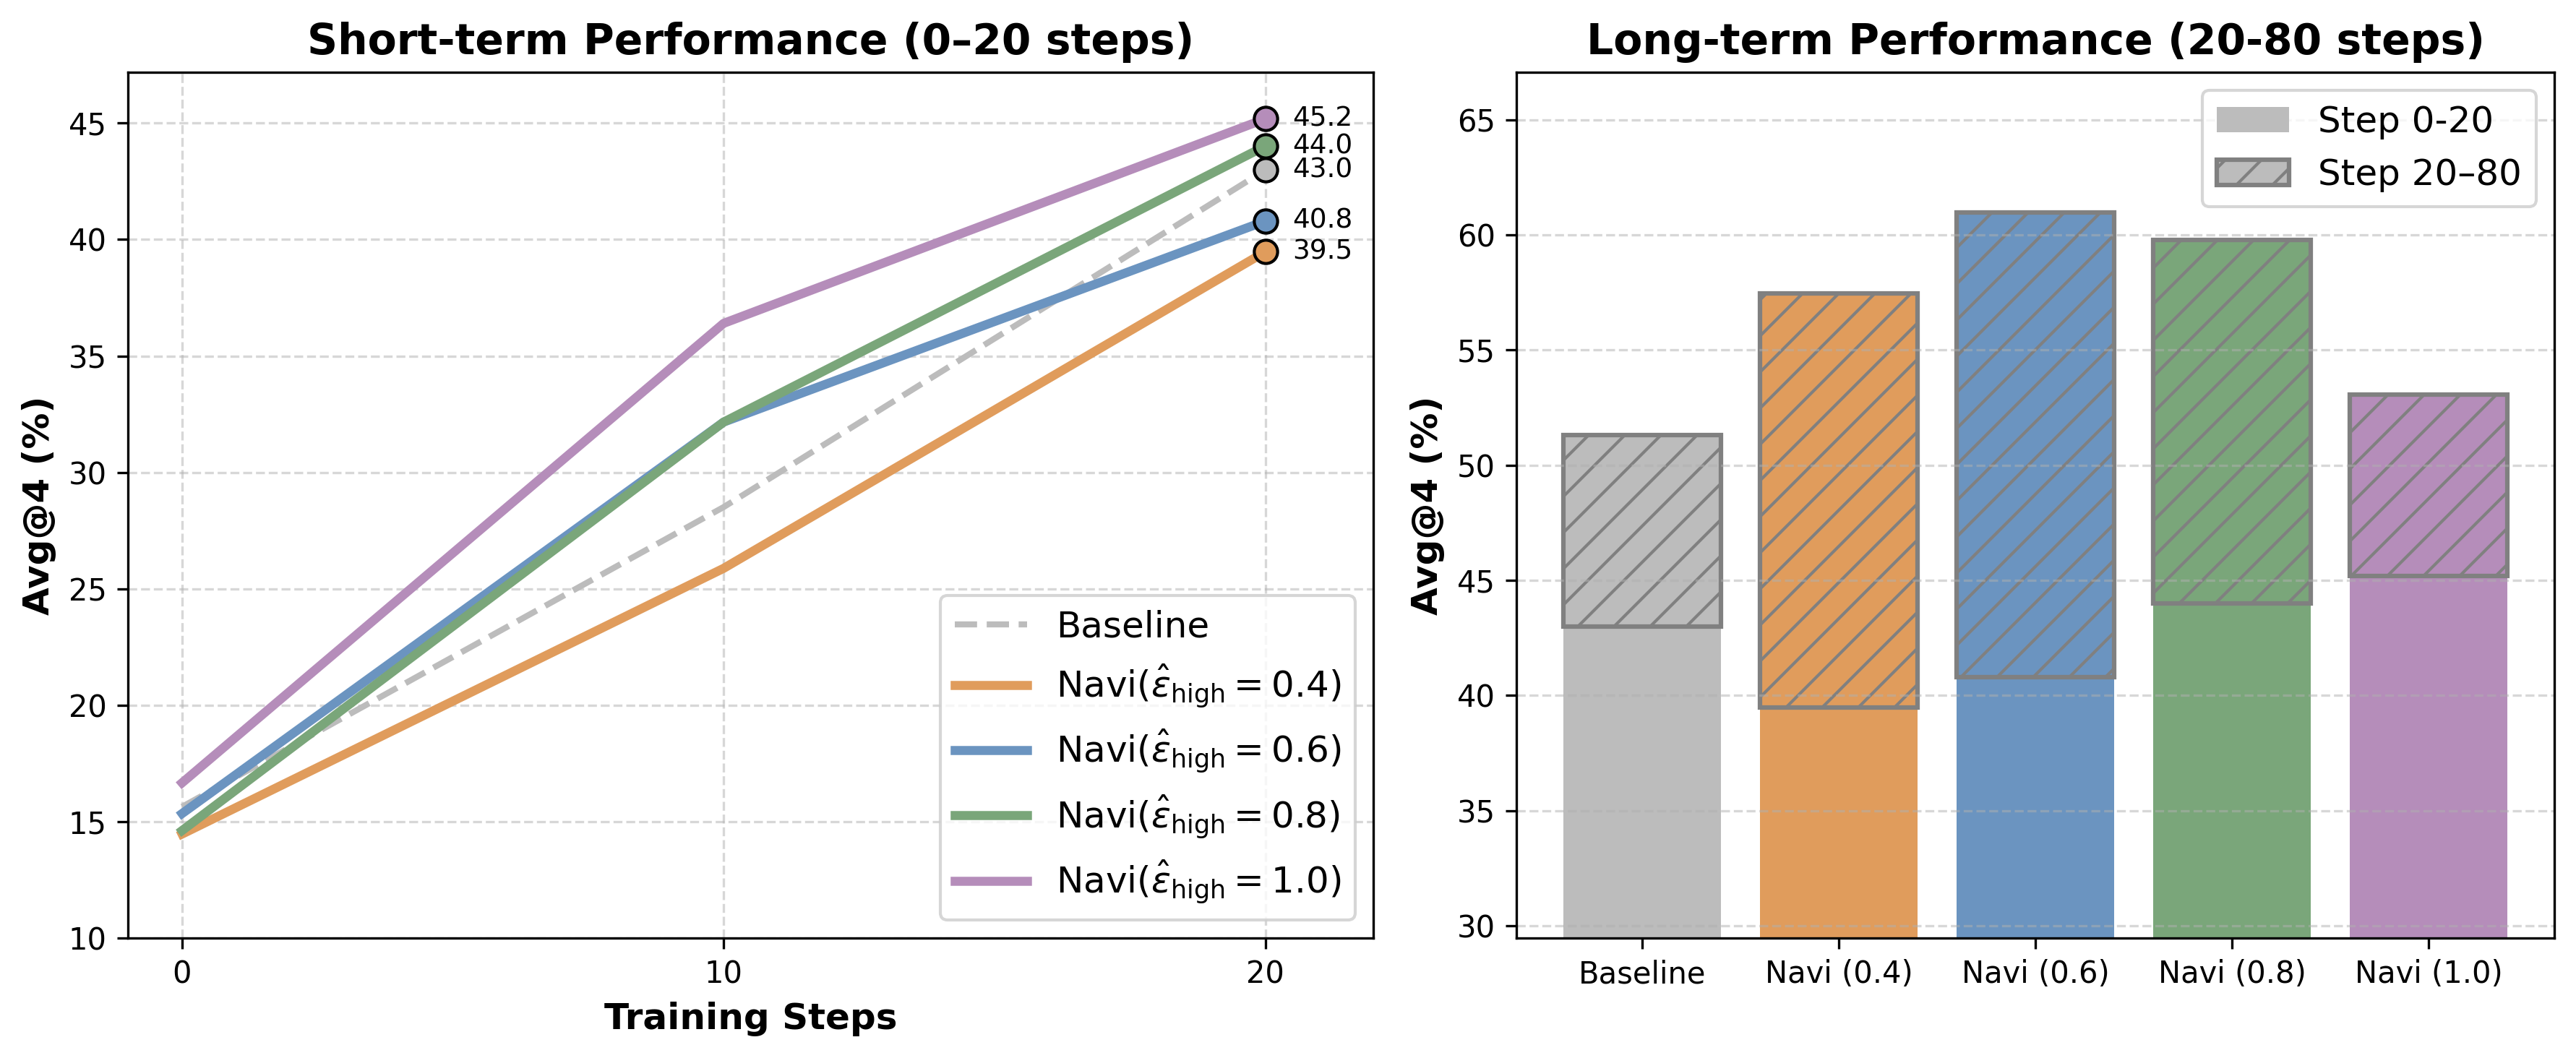
\includegraphics[width=0.85\textwidth]{figs/experiment_self_navigating/navi_short-long-term.png}
  \caption{Impact of $\hat{\epsilon}_{\text{high}}$ on learning dynamics. Higher values speed up early learning but harm long-term performance due to overfitting. A value of $\hat{\epsilon}_{\text{high}}=0.6$ offers the best balance between short- and long-term optimization.
  } 
  \label{fig:navi_short-long-term}
\end{figure}
% =====


\subsubsection{Short-term vs. Long-term Optimization}
We finally examine how the model balances immediate gains with sustained improvement by studying the effect of the parameter $\hat{\epsilon}_{\text{high}}$ in Eq.~\ref{eq:navigating_loss}.
This parameter relaxes the GRPO clipping threshold, mitigating distribution shifts introduced by experience-guided rollouts and preserving valuable positive samples that might otherwise be discarded.
To assess its impact, we vary $\hat{\epsilon}_{\text{high}}$ across the range $\{0.4, 0.6, 0.8, 1.0\}$. As shown in Figure~\ref{fig:navi_short-long-term}, we find that larger values accelerate early learning (within the first 20 steps) but tend to compromise long-term performance (up to 80 steps) due to overfitting to biased trajectories. Our findings indicate that setting $\hat{\epsilon}_{\text{high}}=0.6$ achieves the most favorable balance, facilitating both rapid initial progress and stable long-term optimization.
These observations suggest that \textbf{moderate relaxation fosters early progress while maintaining robustness, whereas overly aggressive values may deliver short-term gains at the cost of long-term generalization.}

\subsection{Results of Self-Attributing}
\label{sec:experiment_self-attributin}
This section evaluates the \texttt{self-attributing} mechanism proposed in Section~\ref{sec:self-attribution}, which assigns fine-grained rewards to trajectory steps based on their contribution. We examine three aspects: effectiveness through ablation studies comparing outcome-only, attribution-only, and dual-channel configurations (Section~\ref{sec:attr_effectiveness}); sample efficiency by analyzing convergence speed and training dynamics (Section~\ref{sec:attr_efficiency}); and the impact of the attribution weight hyperparameter $\alpha$ on learning trajectories (Section~\ref{sec:attr_hyperparameter}). Following the main experimental setup, all models are trained exclusively on synthetic data generated by \texttt{self-questioning}, using Qwen2.5-7B and Qwen2.5-14B as backbone models on AppWorld and BFCL v3 benchmarks.

\subsubsection{Effectiveness of Self-Attributing} 
\label{sec:attr_effectiveness}
To validate the effectiveness of our \texttt{self-attributing} mechanism (Section~\ref{sec:self-attribution}), we conduct systematic ablation studies comparing four configurations on AppWorld and BFCL v3: (i) Backbone, the Qwen2.5 models (7B and 14B) without any reinforcement learning; (ii) \textbf{Attributing}, our complete \texttt{self-attributing} method that integrates both attribution rewards $r^{\text{attr}}$ and outcome rewards $r^{\text{out}}$ with $\alpha{=}0.1$ to balance their contributions; (iii) \textbf{w/o $r^{\text{attr}}$}, an ablation that removes step-wise attribution signals and relies solely on terminal outcome rewards; and (iv) \textbf{w/o $r^{\text{out}}$}, an ablation that excludes terminal rewards and depends exclusively on attribution-based feedback. All variants are evaluated using avg@8 and best@8 metrics under the TGC evaluation protocol (Table~\ref{tab:attributing_Effectiveness}).  Note that AppWorld results are reported on the dev set here, while Table~\ref{tab:main_results} uses the test-normal set.

\begin{table}[h]
\centering
\caption{Effectiveness of \texttt{self-attributing}. Columns show avg@8 and best@8 on the \emph{dev} set for each benchmark, plus their averages (Avg.). All values are in percent (\%). \textbf{Bolded numbers} highlight the best results.}
\label{tab:attributing_Effectiveness}
\small
\setlength{\tabcolsep}{8pt}
\begin{tabular}{@{}ll cc cc cc@{}}
\toprule
\textbf{Model} & \textbf{Params} &
\multicolumn{2}{c}{\textbf{AppWorld}} &
\multicolumn{2}{c}{\textbf{BFCL v3}} &
\multicolumn{2}{c}{\textbf{Avg.}} \\
\cmidrule(lr){3-4}\cmidrule(lr){5-6}\cmidrule(l){7-8}
 & &
avg@8 & best@8  &
avg@8  & best@8  &
avg@8  & best@8  \\
\midrule
Qwen2.5-7B   & 7B   & 3.1 & 9.1 & 29.8 & 42.4 & 16.4 & 25.7  \\
\rowcolor{gray!20}
\textbf{Attributing } & \textbf{7B} & \textbf{38.4} & \textbf{57.1} & \textbf{56.8} & \textbf{65.3} & \textbf{47.6} & \textbf{61.2} \\
 - w/o $\hat{r}^{\text{attr}}$  & 7B & 33.6 & 46.6 & 49.0 & 60.6 & 41.3 & {53.6} \\
 - w/o $\hat{r}^{\text{out}}$ & 7B & 20.2 & 37.5 & 51.3 & 65.2 & {35.7} & {51.4} \\
\midrule
Qwen2.5-14B   & 14B   & 17.8 & 27.7 & 41.8 & 55.3 & 29.8 & 41.5  \\
\rowcolor{gray!20}
\textbf{Attributing} & \textbf{14B} & \textbf{59.2} & \textbf{75.1} & \textbf{64.9} & \textbf{76.3} & \textbf{62.0} & \textbf{75.7} \\
 - w/o $\hat{r}^{\text{attr}}$ & 14B & 54.6 & 71.3 & 60.3 & 72.1 & 57.4 & 71.7 \\
 - w/o $\hat{r}^{\text{out}}$ & 14B &  42.5 & 60.3 & 63.4 & 73.5 & {53.0} & {66.9} \\

\bottomrule
\end{tabular}
\end{table}



Our \texttt{self-attributing} method (Attributing) achieves the best performance across all settings, demonstrating substantial improvements over the baseline. On the 7B model, it attains a macro-average of 47.6\% avg@8, compared to {Qwen2.5}'s 16.4\% and 25.7\% respectively. The 14B model shows even stronger results, reaching 62.0\% avg@8 and 75.7\% best@8, significantly outperforming the baseline's 29.8\% and 41.5\%. On AppWorld specifically, \texttt{self-attributing} improves avg@8 from 3.1\% to 38.4\% on the 7B model and from 17.8\% to 59.2\% on the 14B model, representing dramatic gains of 35.3\% and 41.4\% percentage points respectively.

The ablation studies reveal the complementary necessity of both reward channels. The {w/o $\hat{r}^{\text{attr}}$} variant, relying solely on outcome rewards, achieves reasonable performance but suffers from uniform credit assignment across trajectory steps. More notably, the {w/o $\hat{r}^{\text{out}}$} variant shows that process-level signals alone are insufficient: while it substantially improves over {Qwen2.5}, it consistently underperforms {w/o $\hat{r}^{\text{attr}}$} across both model scales. This indicates that attribution provides valuable intermediate guidance but requires terminal outcomes to ground policy learning toward task objectives. The consistent gains of our complete method validate the dual-channel design: combining independently normalized signals for intermediate step quality ($\hat{r}^{\text{attr}}$) and final outcome effectiveness ($\hat{r}^{\text{out}}$) enables the policy to optimize both the reasoning process and task success.



\subsubsection{Sample Efficiency of Self-Attributing}
\label{sec:attr_efficiency}
\begin{figure}[h!]
\centering
% --- Subfigure (a) for AppWorld ---
\begin{subfigure}[b]{0.48\textwidth}
    \centering
    \includegraphics[width=\textwidth]{figs/experiment_self_attributing/sample_efficiency_appworld.pdf}
    \caption{AppWorld}
    \label{fig:appworld}
\end{subfigure}
% --- Subfigure (b) for BFCL v3 ---
\begin{subfigure}[b]{0.48\textwidth}
    \centering
    \includegraphics[width=\textwidth]{figs/experiment_self_attributing/sample_efficiency_bfcl.pdf}
    \caption{BFCL v3}
    \label{fig:bfclv3}
\end{subfigure}
\caption{\textbf{Efficiency under equal training budgets.} Learning curves on the validation sets of the (a) AppWorld and (b) BFCL v3 benchmarks. Our method, Attributing (solid purple line), is compared against the GRPO baseline (dashed grey line).}
\label{fig:attr_sample_efficiency} 
\end{figure}


Beyond improving final performance (Section~\ref{sec:self-attribution}), we now investigate whether the \texttt{self-attributing} mechanism also enhances sample efficiency—a critical consideration for practical agent training. To this end, we conduct a quantitative analysis from two complementary perspectives: convergence speed, measured by the training steps needed to reach a performance threshold, and overall learning throughput, quantified by the Area Under the Curve (AUC). The learning trajectories are visualized in Figure~\ref{fig:attr_sample_efficiency}, with corresponding metrics for the Qwen2.5-14B model detailed in Table~\ref{tab:attr_efficiency_metrics}.


Our Attributing method demonstrates substantial improvements in both convergence speed and overall training efficiency. To reach 90\% of the baseline's final performance, our method requires only 40 training steps on AppWorld (baseline: 90 steps) and 20 steps on BFCL v3 (baseline: 60 steps), corresponding to reductions of 55\% and 67\% respectively. The method also achieves higher area-under-curve scores: 46.26 compared to 41.03 on AppWorld, and 61.02 compared to 55.78 on BFCL v3. These trends are consistent across both benchmarks, as shown in the learning curves of Figure~\ref{fig:attr_sample_efficiency}.

This efficiency gain arises from fine-grained credit assignment. Step-wise attribution signals $\hat{r}^{\text{attr}}$ provide dense feedback at each decision point, complementing sparse terminal outcomes $\hat{r}^{\text{out}}$ in the composite reward. Each trajectory thus yields richer gradient information, reducing variance and minimizing redundant exploration.


\begin{figure}[t!]
  \begin{minipage}{0.51\linewidth}
    \centering
    \includegraphics[width=0.98\textwidth]{figs/experiment_self_attributing/alpha.pdf}
    \vspace{-6pt}
    \caption{\textbf{Learning curves for different $\alpha$ values} on AppWorld. The dashed line shows the outcome-only baseline; colored lines correspond to Attributing with $\alpha \in \{0.05, 0.10, 0.20, 0.30\}$ (darker to lighter).}
    \label{fig:attr_alpha_curves}
  \end{minipage}
  \hspace{2pt}
\begin{minipage}{0.43\linewidth}
    \centering
    \captionof{table}{\textbf{Sample efficiency metrics} for the Qwen2.5-14B backbone model. Steps@.9 measures the training steps required to reach 90\% of the baseline's best performance (lower is better, ↓).}
    \label{tab:attr_efficiency_metrics}
    \footnotesize
    \begin{threeparttable}
      \setlength{\tabcolsep}{6pt} 
      \renewcommand{\arraystretch}{1.05}
      \begin{tabular}{l cc} 
        \toprule
        \textbf{Model} & \makecell{\textbf{AppWorld} \\ Steps@.9 (↓)} & \makecell{\textbf{BFCL v3} \\ Steps@.9 (↓)} \\
        \midrule
        Baseline & 90 & 60 \\
        \rowcolor{gray!15}
        \textbf{Attributing} & \textbf{40} & \textbf{20} \\
        \bottomrule
      \end{tabular}
      \vspace{2pt}
    \end{threeparttable}
\end{minipage}
  \vspace{-8pt}
\end{figure}

\subsubsection{Hyperparameter Analysis}
\label{sec:attr_hyperparameter}
To understand the trade-off between rapid initial convergence and robust long-term performance, we analyze the hyperparameter $\alpha$ from our composite reward $r^{\text{comp}}$ (Eq.~23). This parameter controls the relative influence of the process-oriented guidance from attribution signals ($\hat{r}^{\text{attr}}$) compared to the objective-driven supervision from terminal outcomes. We systematically evaluate several values for $\alpha \in \{0.05, 0.10, 0.20, 0.30\}$, with the resulting learning curves for the Qwen2.5-14B backbone on AppWorld shown in Figure~\ref{fig:attr_alpha_curves}.

The results reveal a trade-off between early convergence and long-term performance. In the early stage of training, larger $\alpha$ values accelerate learning: $\alpha{=}0.30$ (yellow line) reaches 45\% at 20 steps, while the baseline achieves only 28\%. However, this early advantage does not persist. By the end of training, $\alpha{=}0.30$ degrades to 43\%, falling below all other attribution-based settings. In contrast, $\alpha{=}0.10$ (purple line) and $\alpha{=}0.20$ (pink line) maintain strong performance throughout, converging to approximately 59\%—substantially higher than both the baseline (55\%) and the high-$\alpha$ variant. The setting $\alpha{=}0.05$ (dark purple line) shows more conservative early gains but achieves comparable final performance.

This pattern indicates that excessive reliance on attribution signals can harm long-term learning. Large $\alpha$ provides strong process-level guidance that accelerates initial policy improvement, but may cause overfitting to the LLM judge's heuristic labels rather than true task objectives. Conversely, small $\alpha$ underutilizes the attribution channel, slowing early progress. The optimal range $\alpha{\in}[0.10, 0.20]$ balances exploitation of dense attribution feedback with grounding in outcome-based supervision, yielding both rapid convergence and robust final performance.


\subsection{Effectiveness of Context-Managing Templates}\label{sec:experiment_cmt}

Different context-management strategies substantially influence an agent’s ability to adapt to diverse tasks. 
In this section, we evaluate the effectiveness of the four fundamental Context-Managing Templates (CMTs) introduced in Section~\ref{sec:context-manager}, using the \textit{AppWorld} benchmark and evaluating agent's TGC and Scenario Goal Completion (SGC) metrics. 
All experiments are conducted with the Qwen3-14B model as the underlying policy backbone.

\begin{table}[htbp]
\centering
\caption{
\textbf{Comparison of TGC@4, TGC@8, SGC@4, and SGC@8 metrics across different Context-Managing Templates (CMTs) in the AppWorld benchmark.} 
The base model is Qwen3-14B. 
Higher values indicate better performance (↑).
}
\label{tab:results-cmt}
\small
\setlength{\tabcolsep}{7pt}
\begin{tabular}{@{}l cc cc@{}}
\toprule
\textbf{Context-Managing Template (CMT)} &
\multicolumn{2}{c}{\textbf{TGC}} &
\multicolumn{2}{c}{\textbf{SGC}} \\
\cmidrule(lr){2-3}\cmidrule(lr){4-5}
 & @4 (↑) & @8 (↑) & @4 (↑) & @8 (↑) \\
\midrule
Basic Causal Template                      & 0.435          & 0.506             & 0.268             & 0.375 \\
Reasoning-Augmented Template               & \textbf{0.661} & 0.690             & \textbf{0.500}    & \textbf{0.571} \\
Sliding-Window Template                    & 0.560          & 0.601             & 0.393             & 0.411 \\
Self-Context-Managing Template             & 0.613          & \textbf{0.720}    & \textbf{0.500}    & \textbf{0.607} \\
\bottomrule
\end{tabular}
\end{table}

As shown in Table~\ref{tab:results-cmt}, the \textbf{Self-Context-Managing Template (SCMT)} achieves the best overall performance in the AppWorld benchmark, particularly on the long-horizon metric \textbf{TGC@8}. 
AppWorld requires agents to reason over extensive lists of available tool APIs, where only a small subset is relevant to the current task. 
The SCMT improves efficiency by dynamically compressing or discarding redundant context segments, enabling more focused reasoning and streamlined agent–environment interactions.

The \textbf{Reasoning-Augmented Template (RAT)} ranks second, highlighting the benefit of explicit ``think-before-act'' steps in enhancing the reasoning ability of Qwen3 within complex multi-tool environments. 
The \textbf{Sliding-Window Template (SWT)} performs moderately, as its periodic memory summarization can omit essential dependencies over longer sequences, reducing contextual consistency compared to SCMT. 
Finally, the \textbf{Basic Causal Template (BCT)} provides a simple yet robust baseline but lacks adaptive memory control, leading to lower task completion scores in extended contexts.

